\ylDisplay{Päikesepaneelid} % Ülesande nimi
{Jonathan Kalmus} % Autor
{lõppvoor} % Voor
{2018} % Aasta
{P 3} % Ülesande nr.
{3} % Raskustase
{
% Teema: Elektriõpetus

\ifStatement
Vasakpoolsel joonisel on toodud ühe päikesepaneeli tootmisvõimsus ööpäeva lõikes ning parempoolsel joonisel linna tarbimisvõimsus ööpäeva lõikes. Hinnata, mitu taolist päikesepaneeli on vaja, et katta kogu linna energiavajadus ööpäeva jooksul. Kui suur peab olema minimaalselt linna energiamahuti, et ööpäevast kõikumist tootmise ja tarbimise vahel kompenseerida?
\begin{center}
	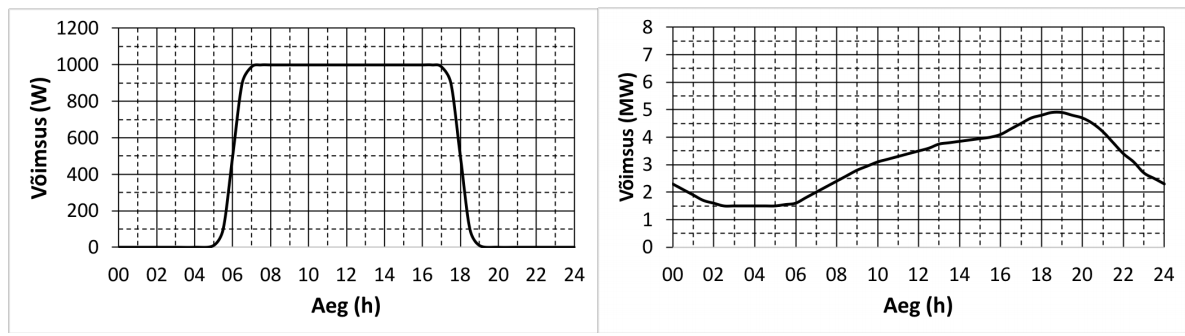
\includegraphics[width=0.5\linewidth]{2018-v3p-03-yl.png}
\end{center}
\fi

\ifHint
Energiamahuti peab suutma talletada kogu päevase ületoodangu ehk selle osa paneelide poolt toodetud energiast, mida linn koheselt ära ei tarbi.
\fi

\ifSolution
\begin{center}
	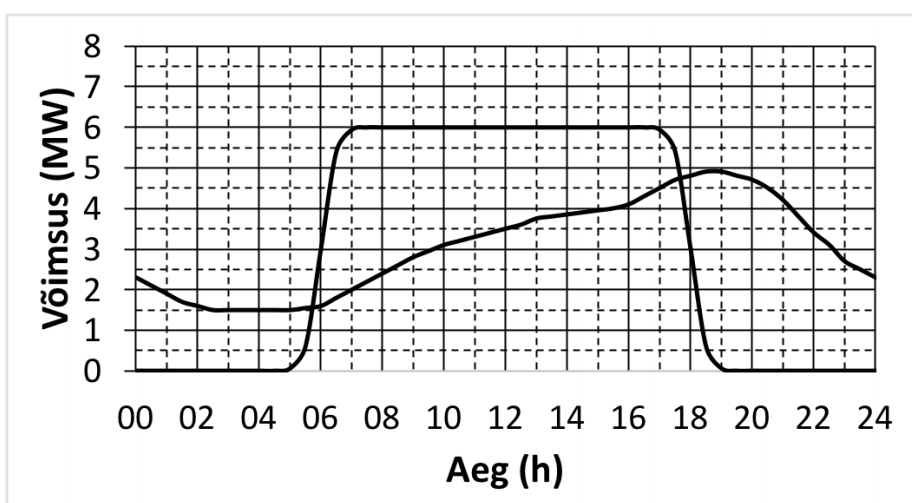
\includegraphics[width=0.5\linewidth]{2018-v3p-03-lah.png}
\end{center}
Päikesepaneeli energiatoodang ööpäeva jooksul on leitav toodud graafiku aluse pindalana, milleks on $E_{paneel} \approx 12$ $kW/h$. Analoogselt on leitav linna energiakulu ööpäevas, milleks on $E_{linn} \approx 74$ $MW/h$. Sellise energiakoguse tootmiseks vajalik paneelide arv $N = \frac{E_{linn}}{E_{paneel}} \approx \frac{74 \cdot 10^6Wh}{12 \cdot 10^3 Wh} \approx 6000$
Energiamahuti peab suutma talletada kogu päevase ületoodangu ehk selle osa $6000$ paneeli poolt toodetud energiast, mida linn koheselt ära ei tarbi. Optimaalse paneelide arvu korral on see ühtlasi võrdne energiaga, mida linn tarbib siis, kui paneelid energiat ei tooda. Selle energia leidmiseks tuleb linna energiatarbimise graafikule visandada $6000$ päikesepaneeli energiatoodangu graafik. Selleks tuleb ühe paneeli graafiku iga punkti väärtus korrutada paneelide arvuga, mille tulemuseks on sama kujuga, kuid $6000$ korda kõrgem graafikuk. Nüüd tuleb lihtsalt leida kas päeval või öösel kahe graafiku vahele jääv pindala, millele vastab energia $E_{mahuti} \approx 30$ $MW/h$, mis ongi vajalik energiamahuti suurus. Olgu öeldud, et sellise süsteemi rajamisel on väga oluline arvestada kõikumistega nii energia tootmises kui tarbimises, mistõttu peaks nii paneelide arv kui enegriamahuti suurus olema kindlasti suuremad kui ülesandes saadud esmane hinnang.
\fi
}